% !TeX spellcheck = ru_RU
% !TEX root = vkr.tex

\section{Обновление библиотеки cuBool и реализация алгоритма}

При первой попытке скомпилировать cuBool (использовались указанные в репозитории команды\footnote{Команды сборки cuBool: \url{https://github.com/SparseLinearAlgebra/cuBool?tab=readme-ov-file\#get-the-source-code-and-run} (Дата посещения: 08.01.2025)} для сборки) возникло большое количество ошибок компиляции.

Была ошибка компиляции связанная с отсутствием включения заголовочного файла стандартной библиотеки C\texttt{++} limits, появившаяся вследствие обновления версии компилятора, следственно и стандартной библиотеки, и скорее всего в gcc-8 он включался в другой заголовочный файл и был доступен без явного его подключения.

Остальные же ошибки были связаны с исходными файлами CUDA, собирающимися компилятором nvcc.
Многие были связаны с отсутствием включения необходимых заголовочных файлов библиотеки thrust, видимо когда-то необходимые функции включались через другие заголовочные файлы. Были ошибки, связанные и с тем, что некоторые файлы перестали существовать, так как они были в detail части thrust (Рис. \ref{fig:CompilerError}).

\begin{figure}[H]
    \centering
    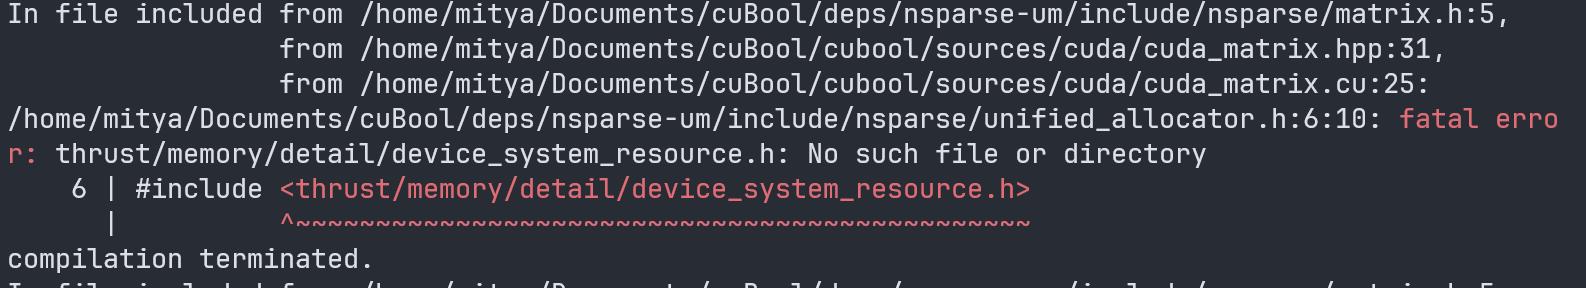
\includegraphics[scale = 0.47]{CompileError.png}
    \caption{Ошибки компиляции из-за отсутствия файлов из detail}
    \label{fig:CompilerError}
\end{figure}

Были же ошибки намного более сложные, они выглядели следующим образом (Рис. \ref{fig:CompilerError2}). Вывод компилятора ничего не говорит о причинах ошибок, он только указывает на отсутствие некоторых синтаксических конструкций, таких как точка с запятой и фигурные скобки. Возможно, это связано с тем, что после стадии препроцессинга получился синтаксически некорректный код, и компилятор не может его распознать как код на C\texttt{++}.

\begin{figure}[H]
    \centering
    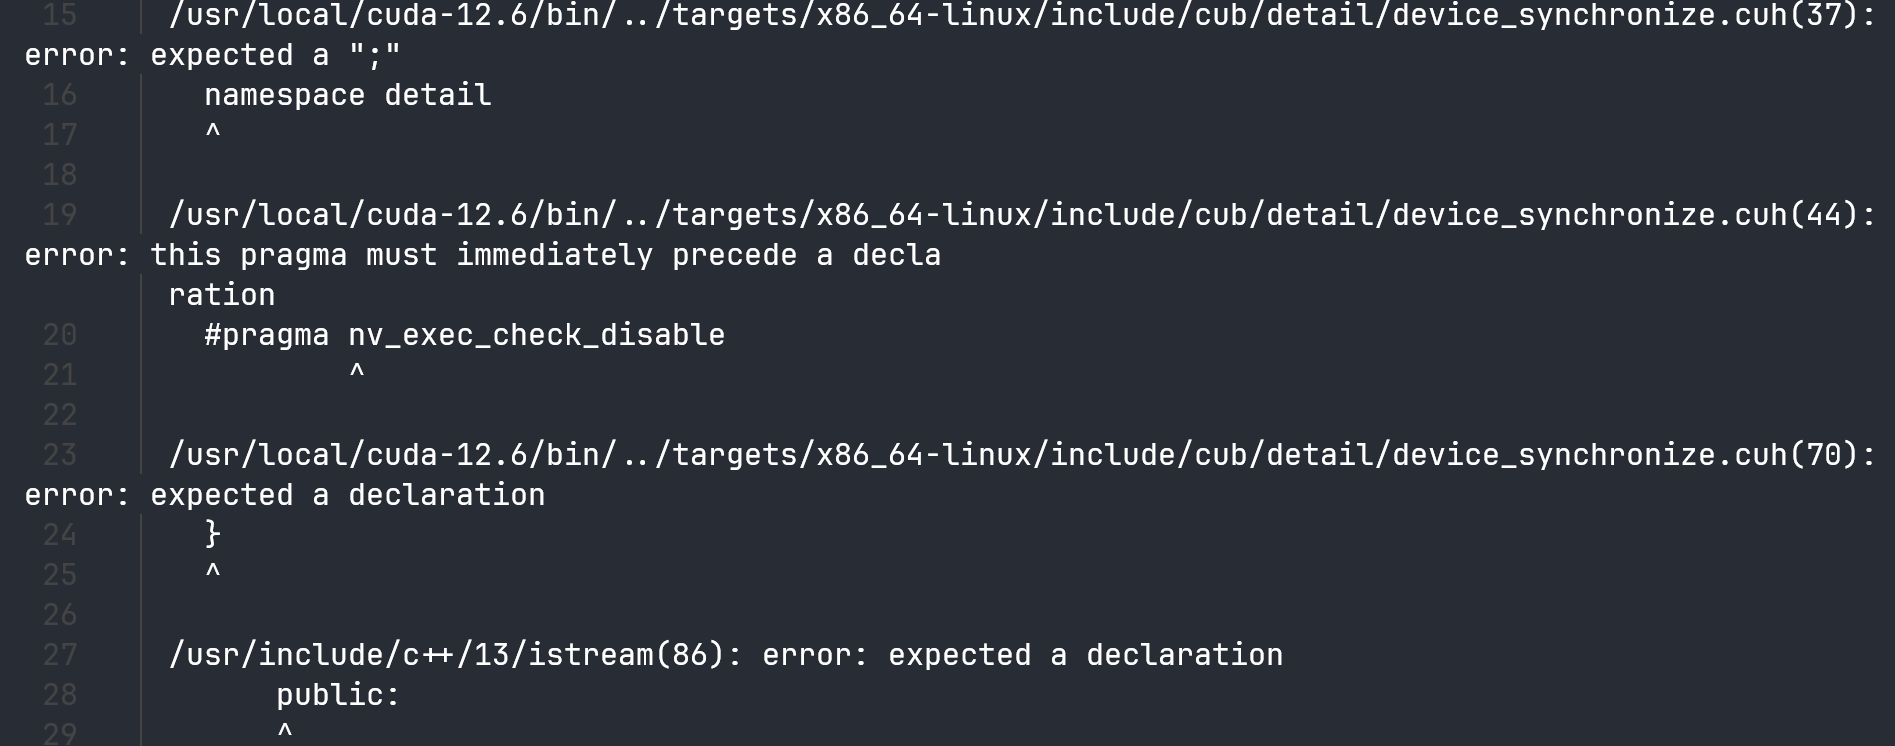
\includegraphics[scale = 0.41]{CompileError2.png}
    \caption{Ошибки компиляции исходных файлов CUDA}
    \label{fig:CompilerError2}
\end{figure}

Можно заметить, что эти ошибки компиляции возникают не в исходных файлах самой библиотеки, а в части Cuda Development Toolkit --- Cub, как можно увидеть на Рис. \ref{fig:CompilerError2}, эти файлы находятся в системе и устанавливаются пакетным менеджером вместе с CUDA. После более подробного изучения cuBool, было обнаружено, что внутри нее тоже есть cub, хотя в последних версиях CUDA он устанавливается вместе с ней. Тогда было удалено включение локального cub в проект, и это помогло скомпилировать библиотеку.

\subsection{Отладка некорректной работы функциональности cuBool}

После компиляции встала задача починить тесты, так как прошло только 101 из 139 тестов. Причины падения тестов были непонятны с первого взгляда,
при этом результат некоторых менялся от запуска к запуску, и иногда они даже проходили.
Во время отладки было обнаружено, что не работает должным образом функция \verb|thrust::set_intersection|.
При пересечении двух массивов, в которых есть одинаковые элементы, она в ответе выдавала пустой массив. Для отладки был создан отдельный проект c простым кодом, использующий эту функцию (Листинг \ref{TestSetIntr}).

\begin{listing}
    \caption{Код для отладки thrust::set\_intersection. Здесь print\_vector --- простая вспомогательная функция, печатающая элементы вектора}
    \begin{minted}[fontsize=\small]{c++}
void test() {
  thrust::device_vector<uint32_t> v {2, 7};
  thrust::device_vector<uint32_t> u {1, 2, 3, 4, 5, 6, 7, 8, 9};
  thrust::device_vector<uint32_t> w(2);

  auto end = thrust::set_intersection(v.begin(), v.end(),
                                      u.begin(), u.end(),
                                      w.begin());
  auto size = thrust::distance(w.begin(), end);

  print_vector(v);
  print_vector(u);
  std::cout << "size = " << size << std::endl;
  print_vector(w);
}
  \end{minted}
\label{TestSetIntr}    
\end{listing}

Этот код работал абсолютно корректно, как от него и ожидалось: в \verb|w| лежали элементы 2 и 7.
Но когда этот код был вставлен в cuBool и вызван в одном из тестов, в ответе опять был пустой массив. После того, как один и тот же код работает по-разному в разных проектах осталось изучать только окружение программы и систему сборки. Окружение было одинаковым, все запускалось с одной машины с одной корневой директорией. Осталось только смотреть на опции сборки.

Более глубокое и подробное изучение CMake у cuBool дало результат. Была найдена опция (Листинг \ref{CmakeOption}), без добавления которой код стал работать корректно и все тесты успешно прошли. Эта опция отвечает за параллельную компиляцию\footnote{
Документация cmake: \url{https://cmake.org/cmake/help/latest/prop_tgt/CUDA_SEPARABLE_COMPILATION.html}
 (Дата посещения: 08.01.2025)} исходных файлов CUDA. Поиск причины ошибки в интернете не дал результатов, так что планируются дальнейшее самостоятельное изучение.  

\begin{listing}
    \caption{Опция CMake, из-за которой thrust работал некорректно}
    \begin{minted}[fontsize=\small]{cmake}
set_target_properties(cubool PROPERTIES CUDA_SEPARABLE_COMPILATION ON)
  \end{minted}
\label{CmakeOption}
\end{listing}

Было проверено как изменилось время компиляции библиотеки после удаления опции. Компилятором для C\texttt{++} файлов был выбран gcc версии 14.2, для файлов CUDA --- nvcc версии 12.6.68. Компиляторам была передана опция \verb|-j1| для теста времени работы в однопоточной компиляции. Использовались команды компиляции, указанные в листинге \ref{CompileCommands}. Для замера времени использовалась команда Unix \verb|time|, итоговое время считалось как сумма работы user и system частей.

Время компиляции без опции составило 113.53, с опцией 115.33. Разница находится в пределе погрешности, итоговое время компиляции осталось таким же.

\begin{listing}
    \caption{Команды для замера времени компиляции}
    \begin{minted}[fontsize=\small]{cmake}
cmake -DCMAKE_BUILD_TYPE=Release -DCUBOOL_BUILD_TESTS=ON -B build -S .
time cmake --build build -j1
  \end{minted}
\label{CompileCommands}
\end{listing}

\subsection{Исправление ошибки в сложении матриц}

\begin{listing}
    \caption{Функция сложения, в которой была обнаружена ошибка}
    \begin{minted}[fontsize=\small]{c++}
class SpMergeFunctor {
public:
  // type definitions
  MatrixType operator()(const MatrixType& a, const MatrixType& b) {
    assert(a.m_rows == b.m_rows);
    assert(a.m_cols == b.m_cols);  
    IndexType rows = a.m_rows;
    IndexType cols = a.m_rows;
    // addition GPU operations
    return MatrixType(std::move(col_result), std::move(rpt_result),
                      rows, cols, vals);
  }
  // class fields
};                      
  \end{minted}
  \label{AddBug}
\end{listing}

В ходе разработки алгоритма была обнаружена ошибка в сложении матриц (это можно заметить на упрощенном коде сложения матриц из библиотеки, представленным в листинге \ref{AddBug}). Переменная \verb|cols| должна быть проинициализирована как \verb|a.m_cols|, a не \verb|a.m_rows|, так как при сложении матриц одинакового размера (это условие уже проверенно выше) размер итоговой матрицы должен быть таким же, как и у исходных матриц.

Эта ошибка была допущена вследствие того, что в тестах cuBool не хватает проверки размерности итоговой матрицы, так что в дальнейшем стоит добавить эту проверку в каждый тест.

\subsection{Реализация поэлементного умножения на инвертированную матрицу}

В cuBool все матрицы, в силу своей разреженности, хранятся как множество пар индексов. Для поиска пересечений множества индексов используется функция \verb|thrust::set_intersection|. Тогда для поиска разности множеств индексов отлично подходит функция \verb|thrust::set_difference|. 

Для поддержки операции поэлементного умножения на инвертированную матрицу в cuBool были реализованы следующие функции, классы и файлы.
\begin{itemize}
    \item C-API интерфейсная функция \verb|cuBool_Matrix_EWiseMulInverted|.
    \item Файл \verb|cuBool_Matrix_EWiseMultInverted.cpp| с реализацией C-API функции.
    \item Абстрактный виртуальный метод \verb|eWiseMultInverted| в классе MatrixBase.
    \item Реализация метода \verb|eWiseMultInverted| в наследнике MatrixBase Matrix.
    \item CUDA файл \verb|cuda_matrix_ewisemult_inverted.cu|
 с реализацией метода \verb|eWiseMultInverted| в наследнике \verb|MatrixBase| \verb|CudaMatrix|.
    \item CUDA kernel \verb|spewisemultinverted.cuh| c классом \verb|SpVectorEWiseMultInverted|, в котором реализованы код вычислений на GPU.
    \item Тесты для C-API интерфейсной функции.
\end{itemize}

Все изменения, которые были сделаны в cuBool можно найти в форке GitHub репозитории\footnote{Форк репозитории cuBool: \url{https://github.com/mitya-y/cuBool/} (Дата посещения: 08.01.2025)} на ветке update-cuda-12.6.

\subsection{Реализация алгоритма на базе библиотеки cuBool}

С помощью обновленной версии cuBool алгоритм достижимости с регулярными ограничениями был реализован на GPU. Реализация опирается на работу~\cite{OldRpqVkr} и реализацию алгоритма в LaGraph\footnote{Репозиторий LaGraph: \url{https://github.com/SparseLinearAlgebra/LAGraph/tree/2-rpq} (Дата посещения: 08.01.2025)}.

Были написаны тесты для проверки корректности работы алгоритма. В качестве входных данных был взят пример из работы~\cite{OldRpqVkr} и данные, на котором тестировалась реализация алгоритма на CPU.

Так же был настроен CI в репозитории алгоритма на GitHub в котором происходит компиляция и запуск тестов, в которых используются непараллельные версии функций cuBool для CPU. Tакже применяется анализатор стиля кода при загрузке изменений.

Результаты работы можно найти в репозитории GitHub\footnote{Репозитория с алгоритмом: \url{https://github.com/mitya-y/rpq} (Дата посещения: 08.01.2025)}.
